\documentclass[11pt]{article}
\usepackage[margin=.65in]{geometry}
\usepackage{lmodern}
\usepackage[T1]{fontenc}
\usepackage{amsmath,amssymb,graphicx,booktabs,array,tabularx,microtype,url}
\usepackage[hidelinks]{hyperref}
\emergencystretch=2em
\graphicspath{{figures/}}
\newcommand{\val}[3]{\csname v#1#2#3\endcsname}
\newcommand{\dval}[2]{\csname d#1#2\endcsname}
\expandafter\def\csname vDG_CORALmacro_f1raw\endcsname{0.805071}
\expandafter\def\csname vDG_CORALaccuracyraw\endcsname{0.818802}
\expandafter\def\csname vDG_CORALbalanced_accuracyraw\endcsname{0.814924}
\expandafter\def\csname vDG_CORALeceraw\endcsname{0.085345}
\expandafter\def\csname vDG_CORALadaptive_eceraw\endcsname{0.084989}
\expandafter\def\csname vDG_CORALnllraw\endcsname{0.619078}
\expandafter\def\csname vDG_CORALbrierraw\endcsname{0.272366}
\expandafter\def\csname vDG_CORALmean_confidenceraw\endcsname{0.902535}
\expandafter\def\csname vDG_CORALconfidence_accuracy_gapraw\endcsname{0.083734}
\expandafter\def\csname vDG_CORALentropyraw\endcsname{0.268331}
\expandafter\def\csname vDG_DANNmacro_f1raw\endcsname{0.800926}
\expandafter\def\csname vDG_DANNaccuracyraw\endcsname{0.814236}
\expandafter\def\csname vDG_DANNbalanced_accuracyraw\endcsname{0.810271}
\expandafter\def\csname vDG_DANNeceraw\endcsname{0.082895}
\expandafter\def\csname vDG_DANNadaptive_eceraw\endcsname{0.082517}
\expandafter\def\csname vDG_DANNnllraw\endcsname{0.628601}
\expandafter\def\csname vDG_DANNbrierraw\endcsname{0.277609}
\expandafter\def\csname vDG_DANNmean_confidenceraw\endcsname{0.895522}
\expandafter\def\csname vDG_DANNconfidence_accuracy_gapraw\endcsname{0.081286}
\expandafter\def\csname vDG_DANNentropyraw\endcsname{0.290740}
\expandafter\def\csname vDG_GROUPDROmacro_f1raw\endcsname{0.761754}
\expandafter\def\csname vDG_GROUPDROaccuracyraw\endcsname{0.777513}
\expandafter\def\csname vDG_GROUPDRObalanced_accuracyraw\endcsname{0.773912}
\expandafter\def\csname vDG_GROUPDROeceraw\endcsname{0.084448}
\expandafter\def\csname vDG_GROUPDROadaptive_eceraw\endcsname{0.084358}
\expandafter\def\csname vDG_GROUPDROnllraw\endcsname{0.694930}
\expandafter\def\csname vDG_GROUPDRObrierraw\endcsname{0.324076}
\expandafter\def\csname vDG_GROUPDROmean_confidenceraw\endcsname{0.858383}
\expandafter\def\csname vDG_GROUPDROconfidence_accuracy_gapraw\endcsname{0.080870}
\expandafter\def\csname vDG_GROUPDROentropyraw\endcsname{0.395285}
\expandafter\def\csname vEMB_STDmacro_f1raw\endcsname{0.828490}
\expandafter\def\csname vEMB_STDaccuracyraw\endcsname{0.835633}
\expandafter\def\csname vEMB_STDbalanced_accuracyraw\endcsname{0.833442}
\expandafter\def\csname vEMB_STDeceraw\endcsname{0.086063}
\expandafter\def\csname vEMB_STDadaptive_eceraw\endcsname{0.085542}
\expandafter\def\csname vEMB_STDnllraw\endcsname{0.602781}
\expandafter\def\csname vEMB_STDbrierraw\endcsname{0.253629}
\expandafter\def\csname vEMB_STDmean_confidenceraw\endcsname{0.920716}
\expandafter\def\csname vEMB_STDconfidence_accuracy_gapraw\endcsname{0.085083}
\expandafter\def\csname vEMB_STDentropyraw\endcsname{0.216653}
\expandafter\def\csname vEMB_STDmacro_f1source_temperature\endcsname{0.828490}
\expandafter\def\csname vEMB_STDaccuracysource_temperature\endcsname{0.835633}
\expandafter\def\csname vEMB_STDbalanced_accuracysource_temperature\endcsname{0.833442}
\expandafter\def\csname vEMB_STDecesource_temperature\endcsname{0.050473}
\expandafter\def\csname vEMB_STDadaptive_ecesource_temperature\endcsname{0.050113}
\expandafter\def\csname vEMB_STDnllsource_temperature\endcsname{0.492366}
\expandafter\def\csname vEMB_STDbriersource_temperature\endcsname{0.236690}
\expandafter\def\csname vEMB_STDmean_confidencesource_temperature\endcsname{0.846658}
\expandafter\def\csname vEMB_STDconfidence_accuracy_gapsource_temperature\endcsname{0.011025}
\expandafter\def\csname vEMB_STDentropysource_temperature\endcsname{0.463513}
\expandafter\def\csname vP0macro_f1raw\endcsname{0.805679}
\expandafter\def\csname vP0accuracyraw\endcsname{0.818769}
\expandafter\def\csname vP0balanced_accuracyraw\endcsname{0.815041}
\expandafter\def\csname vP0eceraw\endcsname{0.088851}
\expandafter\def\csname vP0adaptive_eceraw\endcsname{0.088564}
\expandafter\def\csname vP0nllraw\endcsname{0.630793}
\expandafter\def\csname vP0brierraw\endcsname{0.274186}
\expandafter\def\csname vP0mean_confidenceraw\endcsname{0.906438}
\expandafter\def\csname vP0confidence_accuracy_gapraw\endcsname{0.087670}
\expandafter\def\csname vP0entropyraw\endcsname{0.256117}
\expandafter\def\csname vP0macro_f1source_temperature\endcsname{0.805679}
\expandafter\def\csname vP0accuracysource_temperature\endcsname{0.818769}
\expandafter\def\csname vP0balanced_accuracysource_temperature\endcsname{0.815041}
\expandafter\def\csname vP0ecesource_temperature\endcsname{0.051346}
\expandafter\def\csname vP0adaptive_ecesource_temperature\endcsname{0.051058}
\expandafter\def\csname vP0nllsource_temperature\endcsname{0.533533}
\expandafter\def\csname vP0briersource_temperature\endcsname{0.257165}
\expandafter\def\csname vP0mean_confidencesource_temperature\endcsname{0.836463}
\expandafter\def\csname vP0confidence_accuracy_gapsource_temperature\endcsname{0.017694}
\expandafter\def\csname vP0entropysource_temperature\endcsname{0.487738}
\expandafter\def\csname vP0_WIDEmacro_f1raw\endcsname{0.801535}
\expandafter\def\csname vP0_WIDEaccuracyraw\endcsname{0.815770}
\expandafter\def\csname vP0_WIDEbalanced_accuracyraw\endcsname{0.811932}
\expandafter\def\csname vP0_WIDEeceraw\endcsname{0.099712}
\expandafter\def\csname vP0_WIDEadaptive_eceraw\endcsname{0.099136}
\expandafter\def\csname vP0_WIDEnllraw\endcsname{0.689423}
\expandafter\def\csname vP0_WIDEbrierraw\endcsname{0.283179}
\expandafter\def\csname vP0_WIDEmean_confidenceraw\endcsname{0.914509}
\expandafter\def\csname vP0_WIDEconfidence_accuracy_gapraw\endcsname{0.098739}
\expandafter\def\csname vP0_WIDEentropyraw\endcsname{0.231857}
\expandafter\def\csname vP1macro_f1raw\endcsname{0.809384}
\expandafter\def\csname vP1accuracyraw\endcsname{0.821183}
\expandafter\def\csname vP1balanced_accuracyraw\endcsname{0.817540}
\expandafter\def\csname vP1eceraw\endcsname{0.103895}
\expandafter\def\csname vP1adaptive_eceraw\endcsname{0.103430}
\expandafter\def\csname vP1nllraw\endcsname{0.721163}
\expandafter\def\csname vP1brierraw\endcsname{0.280154}
\expandafter\def\csname vP1mean_confidenceraw\endcsname{0.924395}
\expandafter\def\csname vP1confidence_accuracy_gapraw\endcsname{0.103212}
\expandafter\def\csname vP1entropyraw\endcsname{0.201516}
\expandafter\def\csname vP2macro_f1raw\endcsname{0.806726}
\expandafter\def\csname vP2accuracyraw\endcsname{0.817941}
\expandafter\def\csname vP2balanced_accuracyraw\endcsname{0.814536}
\expandafter\def\csname vP2eceraw\endcsname{0.108310}
\expandafter\def\csname vP2adaptive_eceraw\endcsname{0.107900}
\expandafter\def\csname vP2nllraw\endcsname{0.744285}
\expandafter\def\csname vP2brierraw\endcsname{0.287191}
\expandafter\def\csname vP2mean_confidenceraw\endcsname{0.925649}
\expandafter\def\csname vP2confidence_accuracy_gapraw\endcsname{0.107708}
\expandafter\def\csname vP2entropyraw\endcsname{0.197788}
\expandafter\def\csname vP2macro_f1source_temperature\endcsname{0.806726}
\expandafter\def\csname vP2accuracysource_temperature\endcsname{0.817941}
\expandafter\def\csname vP2balanced_accuracysource_temperature\endcsname{0.814536}
\expandafter\def\csname vP2ecesource_temperature\endcsname{0.050924}
\expandafter\def\csname vP2adaptive_ecesource_temperature\endcsname{0.050447}
\expandafter\def\csname vP2nllsource_temperature\endcsname{0.537034}
\expandafter\def\csname vP2briersource_temperature\endcsname{0.260114}
\expandafter\def\csname vP2mean_confidencesource_temperature\endcsname{0.839290}
\expandafter\def\csname vP2confidence_accuracy_gapsource_temperature\endcsname{0.021349}
\expandafter\def\csname vP2entropysource_temperature\endcsname{0.477056}
\expandafter\def\csname vP2_MISMATCHED_RXmacro_f1raw\endcsname{0.787088}
\expandafter\def\csname vP2_MISMATCHED_RXaccuracyraw\endcsname{0.802328}
\expandafter\def\csname vP2_MISMATCHED_RXbalanced_accuracyraw\endcsname{0.798361}
\expandafter\def\csname vP2_MISMATCHED_RXeceraw\endcsname{0.122491}
\expandafter\def\csname vP2_MISMATCHED_RXadaptive_eceraw\endcsname{0.121926}
\expandafter\def\csname vP2_MISMATCHED_RXnllraw\endcsname{0.864034}
\expandafter\def\csname vP2_MISMATCHED_RXbrierraw\endcsname{0.314737}
\expandafter\def\csname vP2_MISMATCHED_RXmean_confidenceraw\endcsname{0.924203}
\expandafter\def\csname vP2_MISMATCHED_RXconfidence_accuracy_gapraw\endcsname{0.121875}
\expandafter\def\csname vP2_MISMATCHED_RXentropyraw\endcsname{0.201432}
\expandafter\def\csname vP2_NULLmacro_f1raw\endcsname{0.782610}
\expandafter\def\csname vP2_NULLaccuracyraw\endcsname{0.797957}
\expandafter\def\csname vP2_NULLbalanced_accuracyraw\endcsname{0.794084}
\expandafter\def\csname vP2_NULLeceraw\endcsname{0.106905}
\expandafter\def\csname vP2_NULLadaptive_eceraw\endcsname{0.105967}
\expandafter\def\csname vP2_NULLnllraw\endcsname{0.782545}
\expandafter\def\csname vP2_NULLbrierraw\endcsname{0.311458}
\expandafter\def\csname vP2_NULLmean_confidenceraw\endcsname{0.902381}
\expandafter\def\csname vP2_NULLconfidence_accuracy_gapraw\endcsname{0.104424}
\expandafter\def\csname vP2_NULLentropyraw\endcsname{0.264145}
\expandafter\def\csname vP2_SHUFFLEDmacro_f1raw\endcsname{0.788362}
\expandafter\def\csname vP2_SHUFFLEDaccuracyraw\endcsname{0.803866}
\expandafter\def\csname vP2_SHUFFLEDbalanced_accuracyraw\endcsname{0.799788}
\expandafter\def\csname vP2_SHUFFLEDeceraw\endcsname{0.121645}
\expandafter\def\csname vP2_SHUFFLEDadaptive_eceraw\endcsname{0.121200}
\expandafter\def\csname vP2_SHUFFLEDnllraw\endcsname{0.854937}
\expandafter\def\csname vP2_SHUFFLEDbrierraw\endcsname{0.312607}
\expandafter\def\csname vP2_SHUFFLEDmean_confidenceraw\endcsname{0.924928}
\expandafter\def\csname vP2_SHUFFLEDconfidence_accuracy_gapraw\endcsname{0.121062}
\expandafter\def\csname vP2_SHUFFLEDentropyraw\endcsname{0.199756}
\expandafter\def\csname vRX_NORMmacro_f1raw\endcsname{0.800769}
\expandafter\def\csname vRX_NORMaccuracyraw\endcsname{0.814900}
\expandafter\def\csname vRX_NORMbalanced_accuracyraw\endcsname{0.811134}
\expandafter\def\csname vRX_NORMeceraw\endcsname{0.091891}
\expandafter\def\csname vRX_NORMadaptive_eceraw\endcsname{0.091439}
\expandafter\def\csname vRX_NORMnllraw\endcsname{0.643224}
\expandafter\def\csname vRX_NORMbrierraw\endcsname{0.280114}
\expandafter\def\csname vRX_NORMmean_confidenceraw\endcsname{0.905641}
\expandafter\def\csname vRX_NORMconfidence_accuracy_gapraw\endcsname{0.090740}
\expandafter\def\csname vRX_NORMentropyraw\endcsname{0.258960}
\expandafter\def\csname vSAR_GNmacro_f1raw\endcsname{0.805684}
\expandafter\def\csname vSAR_GNaccuracyraw\endcsname{0.818776}
\expandafter\def\csname vSAR_GNbalanced_accuracyraw\endcsname{0.815049}
\expandafter\def\csname vSAR_GNeceraw\endcsname{0.088850}
\expandafter\def\csname vSAR_GNadaptive_eceraw\endcsname{0.088571}
\expandafter\def\csname vSAR_GNnllraw\endcsname{0.630804}
\expandafter\def\csname vSAR_GNbrierraw\endcsname{0.274178}
\expandafter\def\csname vSAR_GNmean_confidenceraw\endcsname{0.906449}
\expandafter\def\csname vSAR_GNconfidence_accuracy_gapraw\endcsname{0.087674}
\expandafter\def\csname vSAR_GNentropyraw\endcsname{0.256090}
\expandafter\def\csname vSAR_GNmacro_f1source_temperature\endcsname{0.805684}
\expandafter\def\csname vSAR_GNaccuracysource_temperature\endcsname{0.818776}
\expandafter\def\csname vSAR_GNbalanced_accuracysource_temperature\endcsname{0.815049}
\expandafter\def\csname vSAR_GNecesource_temperature\endcsname{0.051402}
\expandafter\def\csname vSAR_GNadaptive_ecesource_temperature\endcsname{0.051091}
\expandafter\def\csname vSAR_GNnllsource_temperature\endcsname{0.533526}
\expandafter\def\csname vSAR_GNbriersource_temperature\endcsname{0.257157}
\expandafter\def\csname vSAR_GNmean_confidencesource_temperature\endcsname{0.836465}
\expandafter\def\csname vSAR_GNconfidence_accuracy_gapsource_temperature\endcsname{0.017690}
\expandafter\def\csname vSAR_GNentropysource_temperature\endcsname{0.487745}
\expandafter\def\csname vSOURCE_NORMmacro_f1raw\endcsname{0.805976}
\expandafter\def\csname vSOURCE_NORMaccuracyraw\endcsname{0.819476}
\expandafter\def\csname vSOURCE_NORMbalanced_accuracyraw\endcsname{0.815707}
\expandafter\def\csname vSOURCE_NORMeceraw\endcsname{0.087784}
\expandafter\def\csname vSOURCE_NORMadaptive_eceraw\endcsname{0.087436}
\expandafter\def\csname vSOURCE_NORMnllraw\endcsname{0.625244}
\expandafter\def\csname vSOURCE_NORMbrierraw\endcsname{0.272350}
\expandafter\def\csname vSOURCE_NORMmean_confidenceraw\endcsname{0.905968}
\expandafter\def\csname vSOURCE_NORMconfidence_accuracy_gapraw\endcsname{0.086492}
\expandafter\def\csname vSOURCE_NORMentropyraw\endcsname{0.257201}
\expandafter\def\csname vSUP_FT_FULL_128macro_f1raw\endcsname{0.921811}
\expandafter\def\csname vSUP_FT_FULL_128accuracyraw\endcsname{0.925809}
\expandafter\def\csname vSUP_FT_FULL_128balanced_accuracyraw\endcsname{0.921777}
\expandafter\def\csname vSUP_FT_FULL_128eceraw\endcsname{0.022570}
\expandafter\def\csname vSUP_FT_FULL_128adaptive_eceraw\endcsname{0.021544}
\expandafter\def\csname vSUP_FT_FULL_128nllraw\endcsname{0.240977}
\expandafter\def\csname vSUP_FT_FULL_128brierraw\endcsname{0.110300}
\expandafter\def\csname vSUP_FT_FULL_128mean_confidenceraw\endcsname{0.938220}
\expandafter\def\csname vSUP_FT_FULL_128confidence_accuracy_gapraw\endcsname{0.012411}
\expandafter\def\csname vSUP_FT_FULL_128entropyraw\endcsname{0.181499}
\expandafter\def\csname vSUP_FT_HEAD_128macro_f1raw\endcsname{0.838081}
\expandafter\def\csname vSUP_FT_HEAD_128accuracyraw\endcsname{0.845057}
\expandafter\def\csname vSUP_FT_HEAD_128balanced_accuracyraw\endcsname{0.841501}
\expandafter\def\csname vSUP_FT_HEAD_128eceraw\endcsname{0.064833}
\expandafter\def\csname vSUP_FT_HEAD_128adaptive_eceraw\endcsname{0.064655}
\expandafter\def\csname vSUP_FT_HEAD_128nllraw\endcsname{0.491053}
\expandafter\def\csname vSUP_FT_HEAD_128brierraw\endcsname{0.230260}
\expandafter\def\csname vSUP_FT_HEAD_128mean_confidenceraw\endcsname{0.906855}
\expandafter\def\csname vSUP_FT_HEAD_128confidence_accuracy_gapraw\endcsname{0.061798}
\expandafter\def\csname vSUP_FT_HEAD_128entropyraw\endcsname{0.258408}
\expandafter\def\csname vT3Amacro_f1raw\endcsname{0.833692}
\expandafter\def\csname vT3Aaccuracyraw\endcsname{0.842459}
\expandafter\def\csname vT3Abalanced_accuracyraw\endcsname{0.841423}
\expandafter\def\csname vT3Aeceraw\endcsname{0.102950}
\expandafter\def\csname vT3Aadaptive_eceraw\endcsname{0.102582}
\expandafter\def\csname vT3Anllraw\endcsname{0.501963}
\expandafter\def\csname vT3Abrierraw\endcsname{0.236342}
\expandafter\def\csname vT3Amean_confidenceraw\endcsname{0.753708}
\expandafter\def\csname vT3Aconfidence_accuracy_gapraw\endcsname{-0.088751}
\expandafter\def\csname vT3Aentropyraw\endcsname{0.739732}
\expandafter\def\csname vT3Amacro_f1source_temperature\endcsname{0.833692}
\expandafter\def\csname vT3Aaccuracysource_temperature\endcsname{0.842459}
\expandafter\def\csname vT3Abalanced_accuracysource_temperature\endcsname{0.841423}
\expandafter\def\csname vT3Aecesource_temperature\endcsname{0.047688}
\expandafter\def\csname vT3Aadaptive_ecesource_temperature\endcsname{0.047955}
\expandafter\def\csname vT3Anllsource_temperature\endcsname{0.459254}
\expandafter\def\csname vT3Abriersource_temperature\endcsname{0.223575}
\expandafter\def\csname vT3Amean_confidencesource_temperature\endcsname{0.848251}
\expandafter\def\csname vT3Aconfidence_accuracy_gapsource_temperature\endcsname{0.005791}
\expandafter\def\csname vT3Aentropysource_temperature\endcsname{0.441924}
\expandafter\def\csname dEMB_STD_MINUS_P0ci95_lower\endcsname{0.017466}
\expandafter\def\csname dEMB_STD_MINUS_P0ci95_upper\endcsname{0.028406}
\expandafter\def\csname dEMB_STD_MINUS_P0mean_difference\endcsname{0.022812}
\expandafter\def\csname dEMB_STD_MINUS_P0receiver_count\endcsname{32}
\expandafter\def\csname dEMB_STD_MINUS_P0replicates\endcsname{10000}
\expandafter\def\csname dEMB_STD_MINUS_P0rng_seed\endcsname{20260906}
\expandafter\def\csname dEMB_STD_MINUS_P0p_value\endcsname{0.000010}
\expandafter\def\csname dEMB_STD_MINUS_P0positive\endcsname{32}
\expandafter\def\csname dEMB_STD_MINUS_T3Aci95_lower\endcsname{-0.010351}
\expandafter\def\csname dEMB_STD_MINUS_T3Aci95_upper\endcsname{-0.000118}
\expandafter\def\csname dEMB_STD_MINUS_T3Amean_difference\endcsname{-0.005202}
\expandafter\def\csname dEMB_STD_MINUS_T3Areceiver_count\endcsname{32}
\expandafter\def\csname dEMB_STD_MINUS_T3Areplicates\endcsname{10000}
\expandafter\def\csname dEMB_STD_MINUS_T3Arng_seed\endcsname{20260906}
\expandafter\def\csname dEMB_STD_MINUS_T3Ap_value\endcsname{0.059369}
\expandafter\def\csname dEMB_STD_MINUS_T3Apositive\endcsname{9}
\expandafter\def\csname dSAR_GN_MINUS_P0ci95_lower\endcsname{-0.000013}
\expandafter\def\csname dSAR_GN_MINUS_P0ci95_upper\endcsname{0.000028}
\expandafter\def\csname dSAR_GN_MINUS_P0mean_difference\endcsname{0.000006}
\expandafter\def\csname dSAR_GN_MINUS_P0receiver_count\endcsname{32}
\expandafter\def\csname dSAR_GN_MINUS_P0replicates\endcsname{10000}
\expandafter\def\csname dSAR_GN_MINUS_P0rng_seed\endcsname{20260906}
\expandafter\def\csname dSAR_GN_MINUS_P0p_value\endcsname{0.640194}
\expandafter\def\csname dSAR_GN_MINUS_P0positive\endcsname{3}
\expandafter\def\csname dSAR_GN_MINUS_T3Aci95_lower\endcsname{-0.034528}
\expandafter\def\csname dSAR_GN_MINUS_T3Aci95_upper\endcsname{-0.021933}
\expandafter\def\csname dSAR_GN_MINUS_T3Amean_difference\endcsname{-0.028008}
\expandafter\def\csname dSAR_GN_MINUS_T3Areceiver_count\endcsname{32}
\expandafter\def\csname dSAR_GN_MINUS_T3Areplicates\endcsname{10000}
\expandafter\def\csname dSAR_GN_MINUS_T3Arng_seed\endcsname{20260906}
\expandafter\def\csname dSAR_GN_MINUS_T3Ap_value\endcsname{0.000010}
\expandafter\def\csname dSAR_GN_MINUS_T3Apositive\endcsname{1}
\expandafter\def\csname dSUP_FT_FULL_128_MINUS_P0ci95_lower\endcsname{0.095270}
\expandafter\def\csname dSUP_FT_FULL_128_MINUS_P0ci95_upper\endcsname{0.137720}
\expandafter\def\csname dSUP_FT_FULL_128_MINUS_P0mean_difference\endcsname{0.116132}
\expandafter\def\csname dSUP_FT_FULL_128_MINUS_P0receiver_count\endcsname{32}
\expandafter\def\csname dSUP_FT_FULL_128_MINUS_P0replicates\endcsname{10000}
\expandafter\def\csname dSUP_FT_FULL_128_MINUS_P0rng_seed\endcsname{20260906}
\expandafter\def\csname dSUP_FT_FULL_128_MINUS_P0p_value\endcsname{0.000010}
\expandafter\def\csname dSUP_FT_FULL_128_MINUS_P0positive\endcsname{32}
\expandafter\def\csname dSUP_FT_FULL_128_MINUS_T3Aci95_lower\endcsname{0.070168}
\expandafter\def\csname dSUP_FT_FULL_128_MINUS_T3Aci95_upper\endcsname{0.106789}
\expandafter\def\csname dSUP_FT_FULL_128_MINUS_T3Amean_difference\endcsname{0.088119}
\expandafter\def\csname dSUP_FT_FULL_128_MINUS_T3Areceiver_count\endcsname{32}
\expandafter\def\csname dSUP_FT_FULL_128_MINUS_T3Areplicates\endcsname{10000}
\expandafter\def\csname dSUP_FT_FULL_128_MINUS_T3Arng_seed\endcsname{20260906}
\expandafter\def\csname dSUP_FT_FULL_128_MINUS_T3Ap_value\endcsname{0.000010}
\expandafter\def\csname dSUP_FT_FULL_128_MINUS_T3Apositive\endcsname{31}
\expandafter\def\csname dT3A_MINUS_P0ci95_lower\endcsname{0.022011}
\expandafter\def\csname dT3A_MINUS_P0ci95_upper\endcsname{0.034661}
\expandafter\def\csname dT3A_MINUS_P0mean_difference\endcsname{0.028014}
\expandafter\def\csname dT3A_MINUS_P0receiver_count\endcsname{32}
\expandafter\def\csname dT3A_MINUS_P0replicates\endcsname{10000}
\expandafter\def\csname dT3A_MINUS_P0rng_seed\endcsname{20260903}
\expandafter\def\csname dT3A_MINUS_P0p_value\endcsname{0.000010}
\expandafter\def\csname dT3A_MINUS_P0positive\endcsname{31}

\newcommand{\studytitle}{Unlabeled Receiver Adaptation for RF Fingerprinting Under Unseen-Receiver Shift: An Information-Matched Comparison on WiSig}
\newcommand{\draftnotice}{Internal-review title proposal (human approval pending); post-hoc analyses; not submission-ready}

\title{Receiver Adaptation: Reviewer-Remediation Supplement}
\author{OpenEW-SA Internal Review}
\date{}
\begin{document}\maketitle
\section{Evidence status and complete receiver coverage}
This is a post-hoc baseline-completeness addendum, not the original confirmatory family. The primary V2 result is unchanged. Raw receiver-by-seed metrics and predictions remain in the immutable external analysis package; the portable release includes all receiver averages and complete reliability bin summaries without RF payloads. The full external metric file contains every frozen method, receiver and seed, with no best-seed filtering.
\begin{center}\small\begin{tabular}{lrrrrr}
\toprule
Receiver & P0 & T3A & P2 & SAR-GN & EMB-STD \\
\midrule
1-1 & 0.7944 & 0.8157 & 0.8269 & 0.7944 & 0.8136 \\
1-19 & 0.7080 & 0.7377 & 0.7213 & 0.7080 & 0.7213 \\
1-20 & 0.8032 & 0.8401 & 0.8568 & 0.8032 & 0.8568 \\
13-14 & 0.7209 & 0.7820 & 0.7212 & 0.7209 & 0.7589 \\
13-7 & 0.8249 & 0.8168 & 0.8116 & 0.8249 & 0.8262 \\
14-7 & 0.8728 & 0.9181 & 0.8544 & 0.8728 & 0.9118 \\
18-19 & 0.8116 & 0.8309 & 0.8233 & 0.8116 & 0.8278 \\
18-2 & 0.7609 & 0.7889 & 0.8021 & 0.7609 & 0.7866 \\
19-1 & 0.7673 & 0.8009 & 0.7587 & 0.7671 & 0.7858 \\
19-19 & 0.8589 & 0.9105 & 0.8205 & 0.8589 & 0.8845 \\
19-2 & 0.8154 & 0.8421 & 0.8012 & 0.8154 & 0.8304 \\
19-20 & 0.7889 & 0.7930 & 0.7783 & 0.7889 & 0.8049 \\
2-1 & 0.7815 & 0.7977 & 0.7935 & 0.7815 & 0.8081 \\
2-19 & 0.8560 & 0.8791 & 0.8570 & 0.8560 & 0.8849 \\
20-1 & 0.9150 & 0.9263 & 0.9279 & 0.9150 & 0.9205 \\
20-19 & 0.8840 & 0.9065 & 0.8460 & 0.8840 & 0.8914 \\
20-20 & 0.7642 & 0.8000 & 0.7821 & 0.7642 & 0.7880 \\
23-1 & 0.9151 & 0.9286 & 0.9141 & 0.9151 & 0.9190 \\
23-3 & 0.8560 & 0.8825 & 0.8463 & 0.8560 & 0.8957 \\
23-5 & 0.8241 & 0.8421 & 0.8060 & 0.8241 & 0.8362 \\
23-6 & 0.9012 & 0.9320 & 0.9160 & 0.9012 & 0.9306 \\
23-7 & 0.7094 & 0.7270 & 0.7476 & 0.7094 & 0.7553 \\
24-13 & 0.8252 & 0.8673 & 0.8553 & 0.8255 & 0.8892 \\
24-16 & 0.8843 & 0.9458 & 0.8524 & 0.8844 & 0.9089 \\
24-5 & 0.5598 & 0.6026 & 0.5765 & 0.5598 & 0.5753 \\
24-6 & 0.8844 & 0.8955 & 0.8885 & 0.8844 & 0.8973 \\
3-19 & 0.6175 & 0.7025 & 0.6054 & 0.6174 & 0.6731 \\
7-14 & 0.7623 & 0.7792 & 0.7547 & 0.7623 & 0.7682 \\
7-7 & 0.8909 & 0.9031 & 0.8908 & 0.8909 & 0.9006 \\
8-14 & 0.7060 & 0.7340 & 0.6786 & 0.7060 & 0.7306 \\
8-7 & 0.8248 & 0.8384 & 0.8152 & 0.8248 & 0.8334 \\
8-8 & 0.8927 & 0.9110 & 0.8853 & 0.8927 & 0.8967 \\
\bottomrule\end{tabular}
\end{center}
\section{Exploratory paired estimates}
Five seeds are averaged within receiver. Bootstrap and sign-flip settings are fixed. No new Holm family is introduced. The full-network method is a label-dependent diagnostic, not an unlabeled competitor.
\begin{center}\small\begin{tabular}{lrrrr}
\toprule
Post-hoc comparison & Delta & 95\% interval & +rx & p \\
\midrule
EMB-STD - P0 & 0.02281 & [0.01747, 0.02841] & 32 & 0.00001 \\
EMB-STD - T3A & -0.00520 & [-0.01035, -0.00012] & 9 & 0.05937 \\
SAR-GN - P0 & 0.00001 & [-0.00001, 0.00003] & 3 & 0.64019 \\
SAR-GN - T3A & -0.02801 & [-0.03453, -0.02193] & 1 & 0.00001 \\
SUP-FT-FULL-128 - P0 & 0.11613 & [0.09527, 0.13772] & 32 & 0.00001 \\
SUP-FT-FULL-128 - T3A & 0.08812 & [0.07017, 0.10679] & 31 & 0.00001 \\
\bottomrule\end{tabular}
\end{center}
\section{Information and implementation details}
P0/P0-WIDE/DG use source labels; T3A and P2 use the frozen unlabeled support bank. SAR-GN updates only GroupNorm affine parameters. EMB-STD uses source-training and target-support moments, retaining the classifier. Full-network supervised FT uses support labels. No query packet participates in adaptation. Transmitter labels are opened only for metrics except in the explicitly labeled oracle branch.

The original SAR fidelity check comprised ten separate synthetic single-update noncollapse cases, not a full ten-minibatch run. The closure state-machine tests additionally cover reset, empty-filter, SAM perturbation, momentum/EMA and receiver isolation, with any official-code deviation recorded separately. At support 128 the frozen 160 records attempted/completed 320 minibatch updates with 293 resets; 146 records reset twice. Replayed final adapted tensors and blind probabilities exactly match the source P0 in 147 records, while 25 receiver-averaged macro-F1 values tie P0. These are different identity claims. This short-support result does not exhaust SAR settings. A separate source-validation-only sensitivity grid compared thresholds 0.2 and the post-hoc normalized-threshold hypothesis over 1, 5 and 20 passes. The latter sharply reduced resets but mean source-validation macro-F1 changed only slightly and nonmonotonically; no new held-out query was evaluated.

The timing replay uses seed 829, all receivers and three repeats. Its total-throughput column is query count divided by total wall time; the legacy internal samples-per-second field has method-specific scopes and is not used for cross-method throughput. Resident models contribute to peak memory. T3A prototype construction is not isolated from query scoring in the total measurement. No timing result replaces a frozen scientific prediction.

\section{Post-hoc oracle composition source and scope}
The main-text POST-HOC ORACLE COMPOSITION DIAGNOSTIC table combines frozen V2 natural-support receiver--seed results with the frozen mechanism-addendum oracle results. The latter combine P2 and T3A/RX-NORM condition files. Exact source filenames, SHA256 hashes, derived summary, and query reconstruction checks appear in the versioned closure evidence report. No new model inference was run for this table.

For each method and condition, five seed macro-F1 values are first averaged inside each of 32 physical receivers; the reported mean gives equal weight to the receivers. Every condition covers 738,015 of 738,015 receiver-seed query records. The frozen P2, T3A and RX-NORM natural prediction archives all match the deterministic query reconstruction (480/480 archives). The original oracle CSVs record query counts but not per-query IDs. The frozen P2 and TTA diagnostic code constructs those rows from the same label-free support/query function and split, which supports the query-alignment claim; direct archived oracle-ID comparison is unavailable.

Natural T3A and RX-NORM use the full 128-packet bank, while natural P2 uses 32 peers drawn from it. Every oracle condition selects at most 32 peers from that same bank. Same-class-excluded and same-class-only select different support for each query using its true transmitter label. Transmitter-pure selects one labeled support class by a fixed hash without consulting test performance. Same-class-only has roughly 21--25 mean peers per receiver-seed record; transmitter-pure can have as few as one. Thus natural-to-oracle differences mix class composition with support amount for T3A/RX-NORM. Oracle conditions are nondeployable, post-hoc diagnostics. Neither EMB-STD nor SAR-GN was evaluated with these oracle supports.

\section{All-receiver reliability}
The following pages cover all 32 receivers for both raw and source-temperature probabilities, always in the same receiver order. Five seed prediction populations are combined within a receiver for descriptive bins. Main-text scalar metrics first average seeds and then receivers. Curves with little bin mass should not be overinterpreted; exact bin mass accompanies the release.
\clearpage
\noindent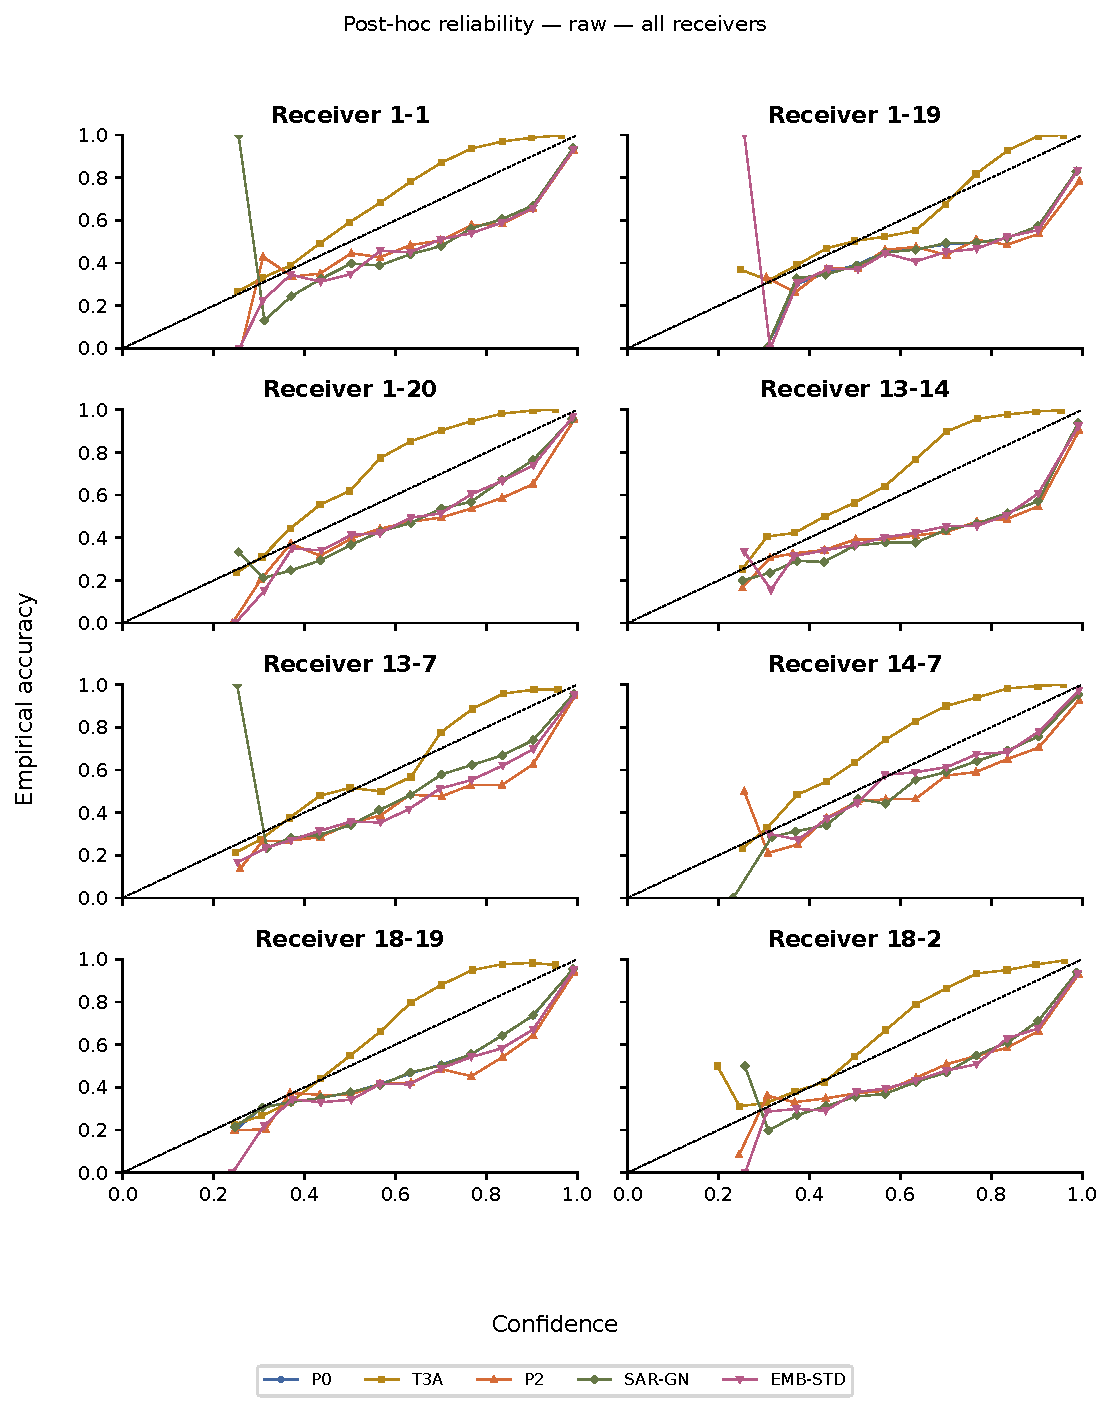
\includegraphics[width=\textwidth,height=.92\textheight,keepaspectratio]{reliability_raw_1}
\clearpage
\noindent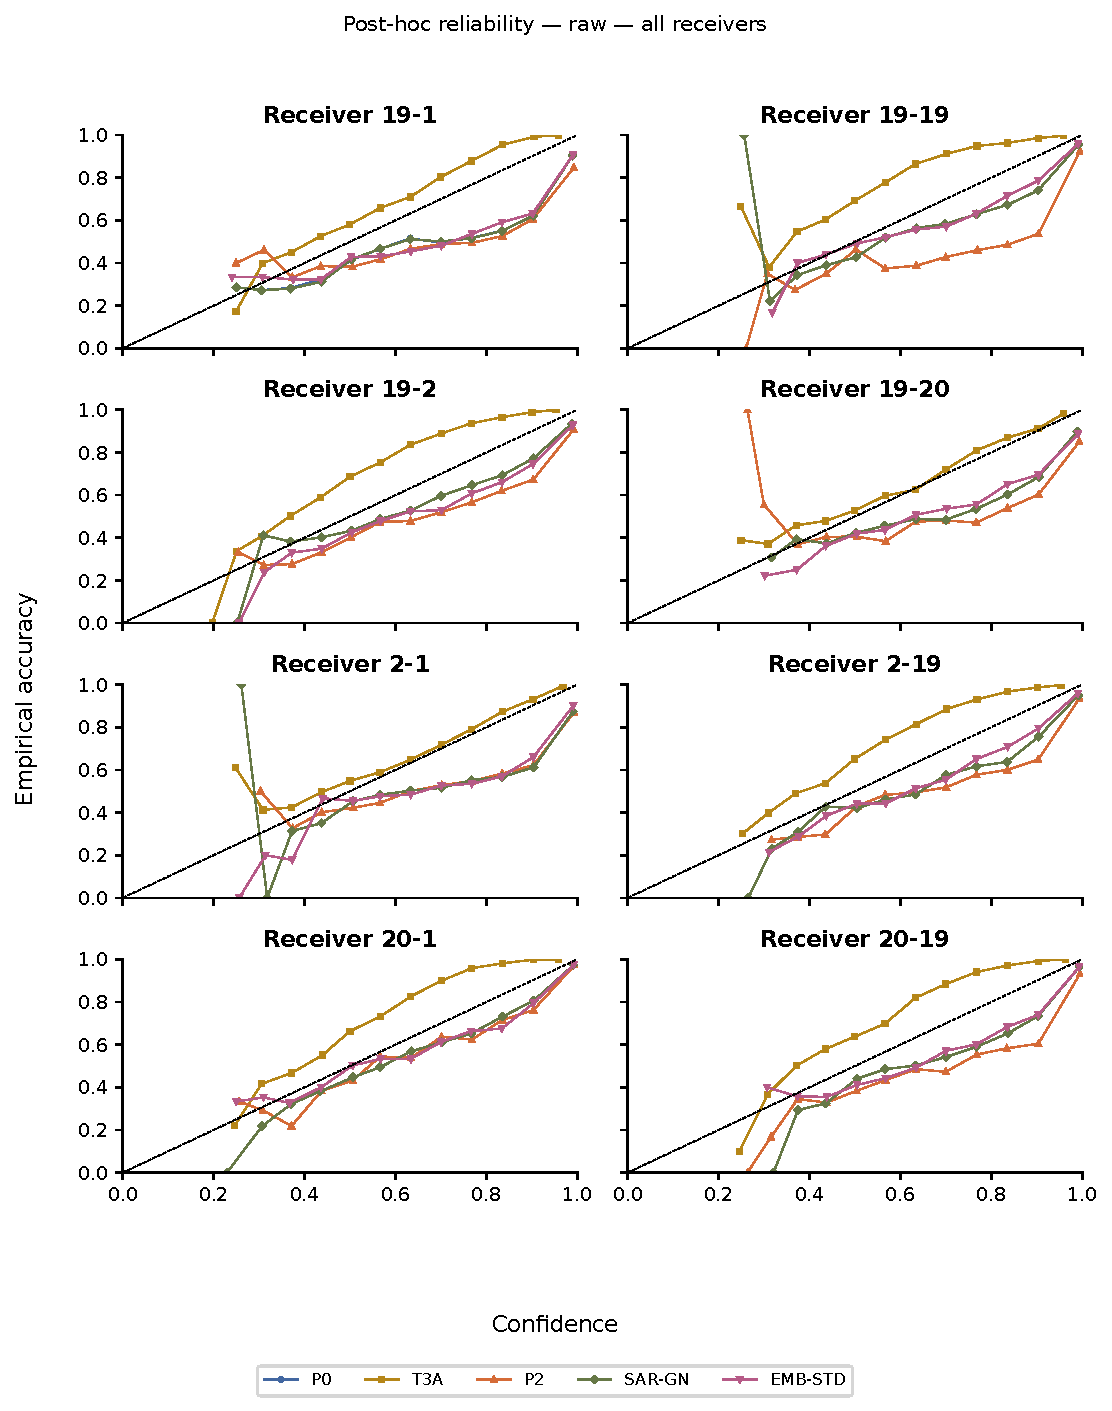
\includegraphics[width=\textwidth,height=.92\textheight,keepaspectratio]{reliability_raw_2}
\clearpage
\noindent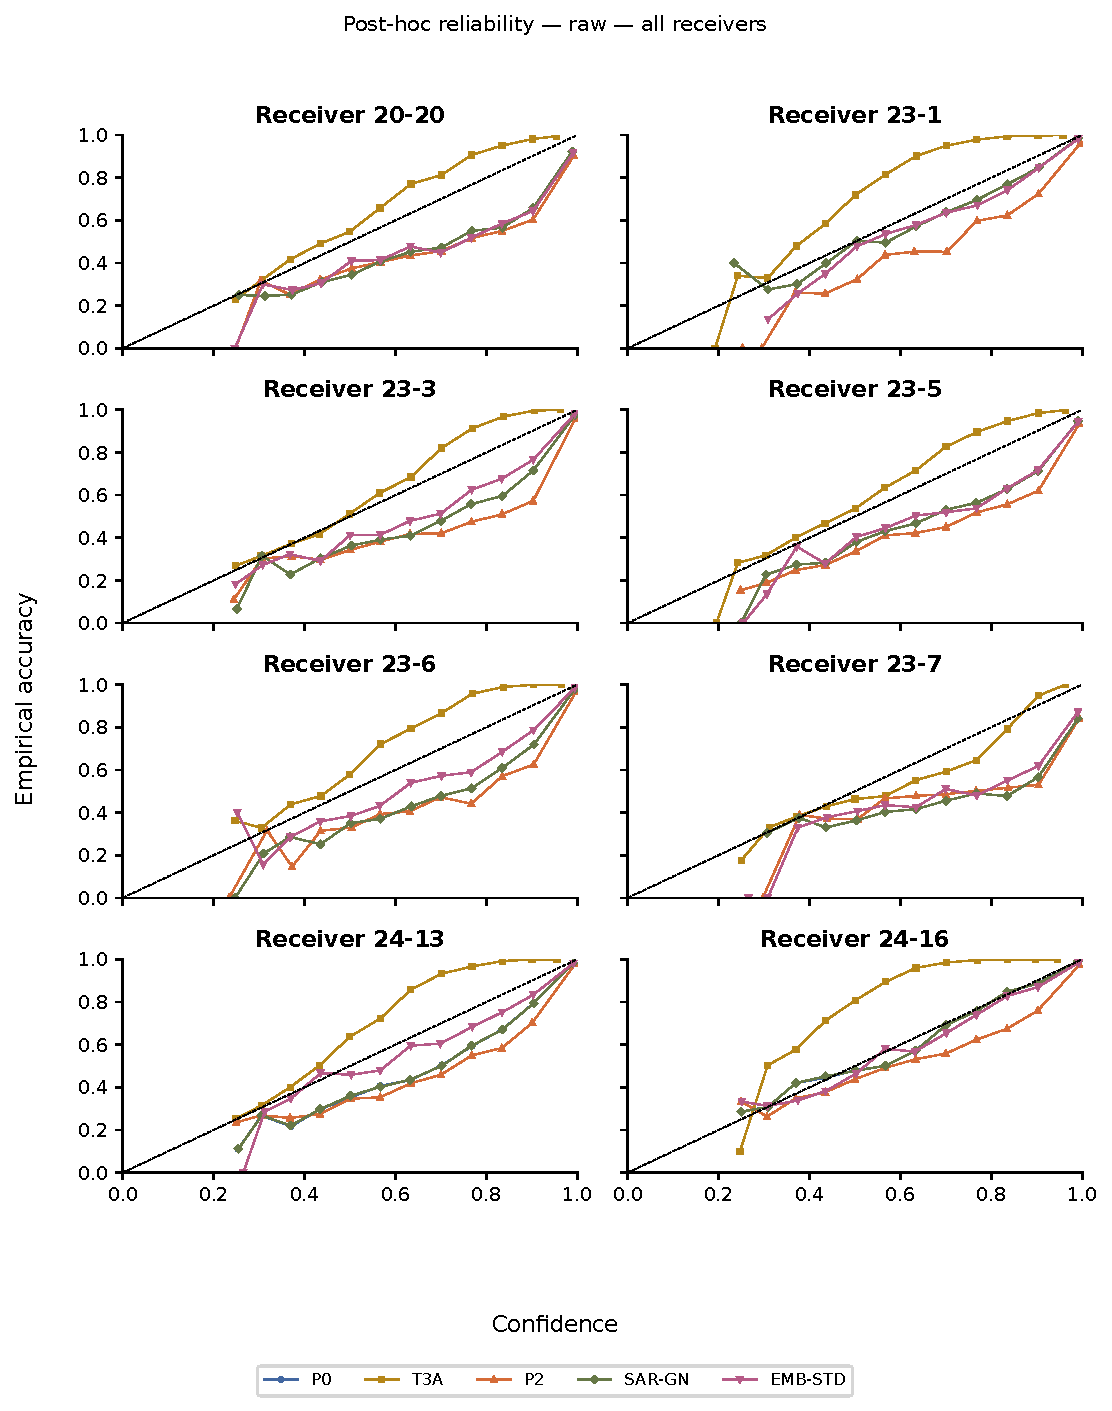
\includegraphics[width=\textwidth,height=.92\textheight,keepaspectratio]{reliability_raw_3}
\clearpage
\noindent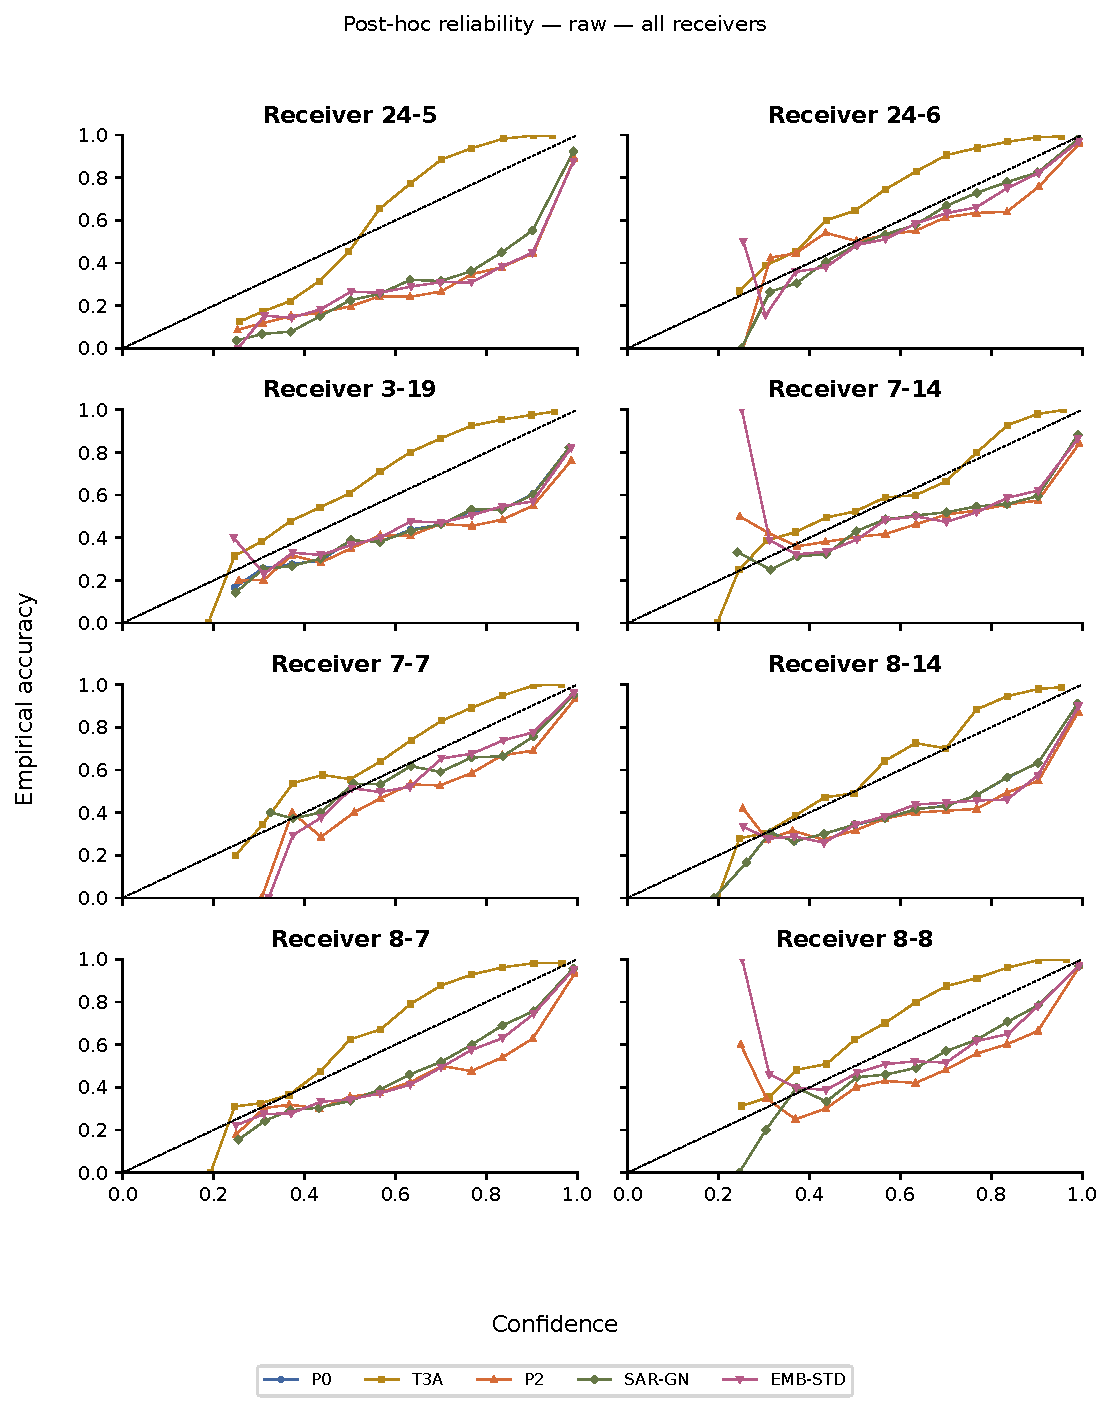
\includegraphics[width=\textwidth,height=.92\textheight,keepaspectratio]{reliability_raw_4}
\clearpage
\noindent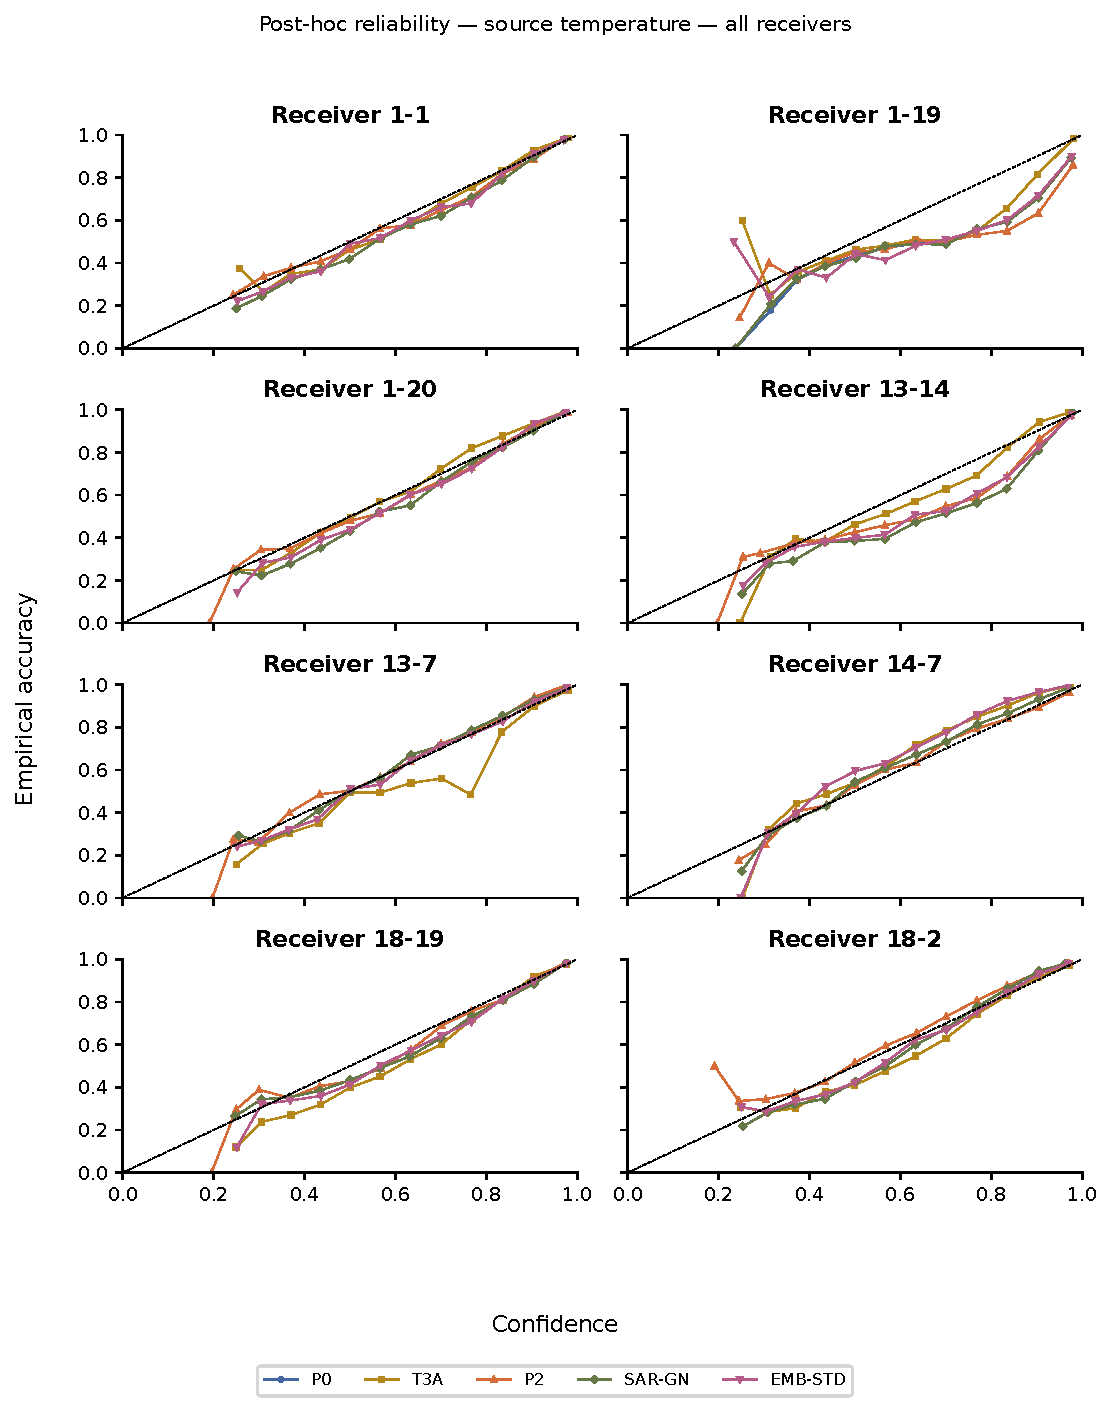
\includegraphics[width=\textwidth,height=.92\textheight,keepaspectratio]{reliability_source_temperature_1}
\clearpage
\noindent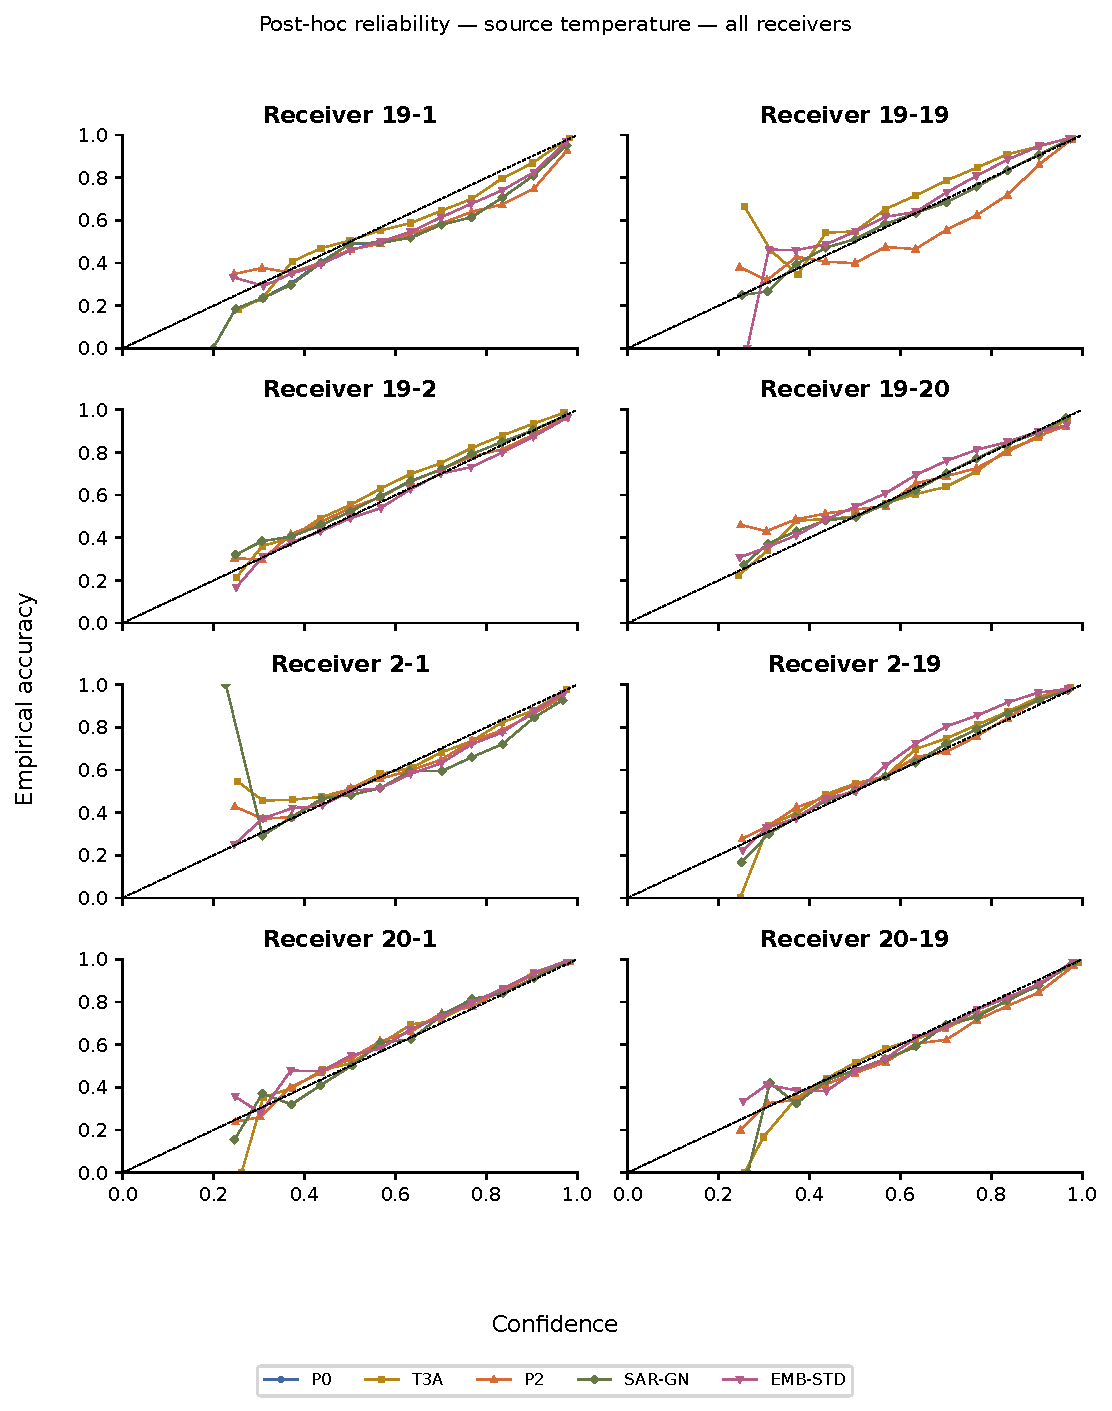
\includegraphics[width=\textwidth,height=.92\textheight,keepaspectratio]{reliability_source_temperature_2}
\clearpage
\noindent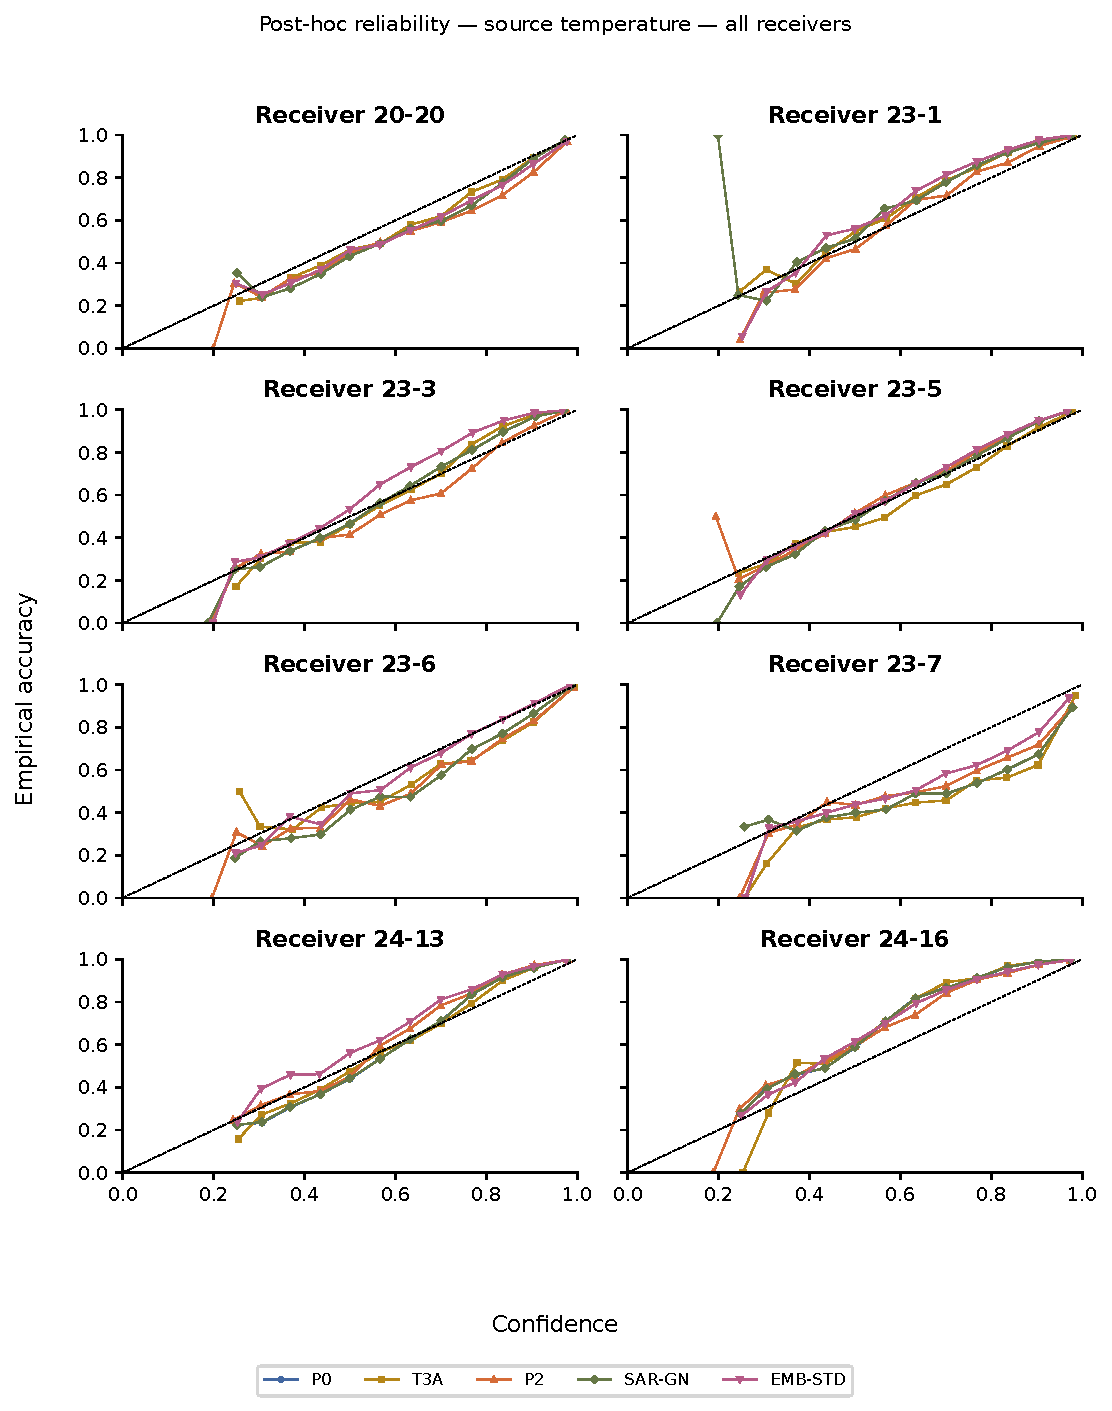
\includegraphics[width=\textwidth,height=.92\textheight,keepaspectratio]{reliability_source_temperature_3}
\clearpage
\noindent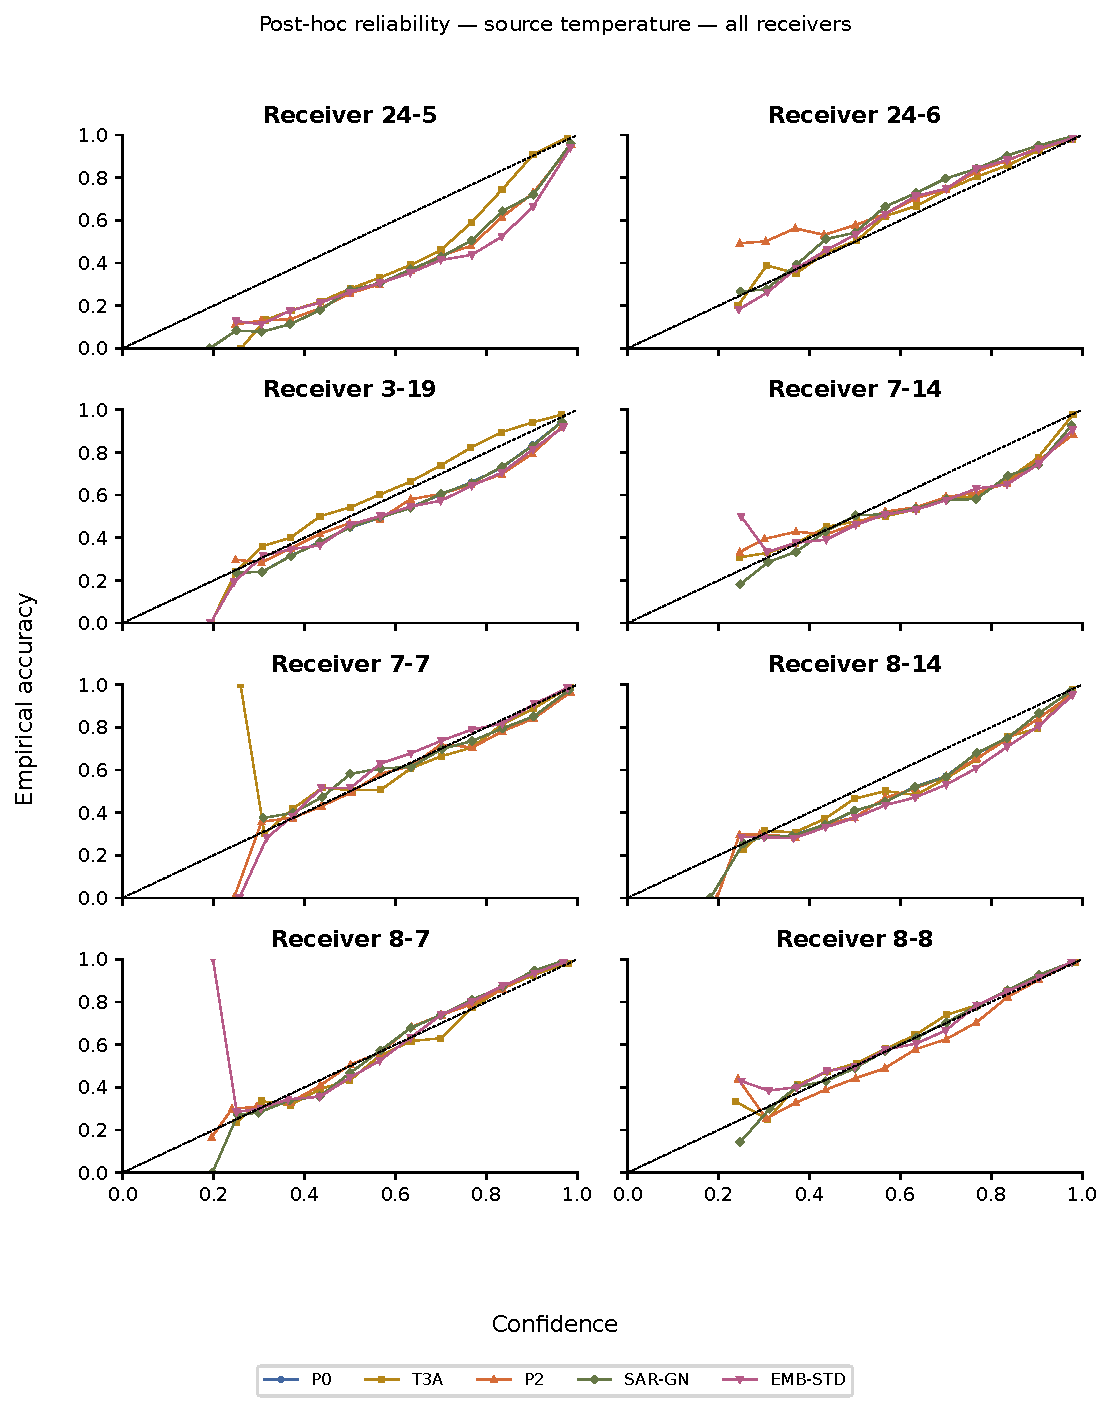
\includegraphics[width=\textwidth,height=.92\textheight,keepaspectratio]{reliability_source_temperature_4}
\clearpage
\end{document}
